\documentclass[tikz]{standalone}

\usepackage{amsfonts}
\usepackage{amsmath}
\usepackage{braket}

\usepackage{tikz}
\usetikzlibrary{calc, decorations, positioning}

\definecolor{googleR}{HTML}{DB4437}
\definecolor{googleG}{HTML}{0F9D58}
\definecolor{googleB}{HTML}{4285F4}

% Main Document
\begin{document}
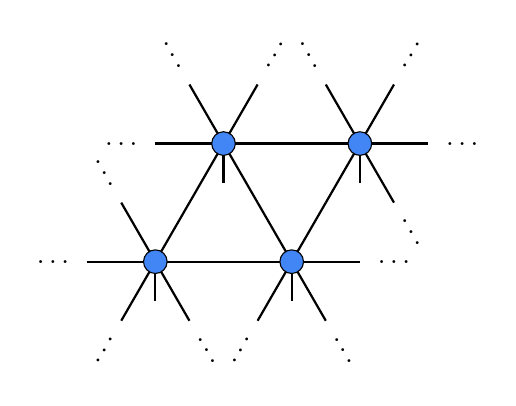
\begin{tikzpicture}
  \def\clipX{2.00}
  \def\clipY{1.75}
  \def\legLength{0.175}
  \def\tensorSize{0.15}
  \def\tensorShiftY{0.0}

  % ------------------------
  % triangular lattice sites
  % ------------------------

  % define coordinates for the triangular lattice
  \coordinate (T1) at ({-1.0*cos(30)}, {+2.0*cos(30)*tan(60)/2});
  \coordinate (T2) at ({+1.0*cos(30)}, {+2.0*cos(30)*tan(60)/2});
  \coordinate (T3) at ({-2.0*cos(30)}, {+0.0*cos(30)*tan(60)/2});
  \coordinate (T4) at ({-0.0*cos(30)}, {+0.0*cos(30)*tan(60)/2});
  \coordinate (T5) at ({+2.0*cos(30)}, {+0.0*cos(30)*tan(60)/2});
  \coordinate (T6) at ({-1.0*cos(30)}, {-2.0*cos(30)*tan(60)/2});
  \coordinate (T7) at ({+1.0*cos(30)}, {-2.0*cos(30)*tan(60)/2});

  \coordinate (C1) at ($(T1) + ({-0.5*cos(30)}, {+1.0*cos(30)*tan(60)/2})$);
  \coordinate (T1b) at ($(T1) + ({+0.5*cos(30)}, {+1.0*cos(30)*tan(60)/2})$);
  \coordinate (T1a) at ($(T2) + ({-0.5*cos(30)}, {+1.0*cos(30)*tan(60)/2})$);
  \coordinate (C2) at ($(T2) + ({+0.5*cos(30)}, {+1.0*cos(30)*tan(60)/2})$);
  \coordinate (T2b) at ($(T2) + ({+1.0*cos(30)}, 0)$);
  \coordinate (T2a) at ($(T5) + ({+0.5*cos(30)}, {+1.0*cos(30)*tan(60)/2})$);
  \coordinate (C3) at ($(T5) + ({+1.0*cos(30)}, 0)$);
  \coordinate (T3b) at ($(T5) + ({+0.5*cos(30)}, {-1.0*cos(30)*tan(60)/2})$);
  \coordinate (T3a) at ($(T7) + ({+1.0*cos(30)}, 0)$);
  \coordinate (C4) at ($(T7) + ({+0.5*cos(30)}, {-1.0*cos(30)*tan(60)/2})$);
  \coordinate (T4b) at ($(T7) + ({-0.5*cos(30)}, {-1.0*cos(30)*tan(60)/2})$);
  \coordinate (T4a) at ($(T6) + ({+0.5*cos(30)}, {-1.0*cos(30)*tan(60)/2})$);
  \coordinate (C5) at ($(T6) + ({-0.5*cos(30)}, {-1.0*cos(30)*tan(60)/2})$);
  \coordinate (T5b) at ($(T6) + ({-1.0*cos(30)}, 0)$);
  \coordinate (T5a) at ($(T3) + ({-0.5*cos(30)}, {-1.0*cos(30)*tan(60)/2})$);
  \coordinate (C6) at ($(T3) + ({-1.0*cos(30)}, 0)$);
  \coordinate (T6b) at ($(T3) + ({-0.5*cos(30)}, {+1.0*cos(30)*tan(60)/2})$);
  \coordinate (T6a) at ($(T1) + ({-1.0*cos(30)}, 0)$);

  \node at ($(T1) + ({-1.50*cos(30)}, {-0.0*cos(30)*tan(60)/2})$) {$\hdots$};
  \node[rotate = -60] at ($(T1) + ({-0.75*cos(30)}, {+1.5*cos(30)*tan(60)/2})$) {$\hdots$};
  \node[rotate = +60] at ($(T1) + ({+0.75*cos(30)}, {+1.5*cos(30)*tan(60)/2})$) {$\hdots$};

  \node at ($(T2) + ({+1.50*cos(30)}, {-0.0*cos(30)*tan(60)/2})$) {$\hdots$};
  \node[rotate = -60] at ($(T2) + ({-0.75*cos(30)}, {+1.5*cos(30)*tan(60)/2})$) {$\hdots$};
  \node[rotate = +60] at ($(T2) + ({+0.75*cos(30)}, {+1.5*cos(30)*tan(60)/2})$) {$\hdots$};
  \node[rotate = -60] at ($(T2) + ({+0.75*cos(30)}, {-1.5*cos(30)*tan(60)/2})$) {$\hdots$};

  \node[rotate = -60] at ($(T3) + ({-0.75*cos(30)}, {+1.5*cos(30)*tan(60)/2})$) {$\hdots$};
  \node at ($(T3) + ({-1.50*cos(30)}, {-0.0*cos(30)*tan(60)/2})$) {$\hdots$};
  \node[rotate = -60] at ($(T3) + ({+0.75*cos(30)}, {-1.5*cos(30)*tan(60)/2})$) {$\hdots$};
  \node[rotate = +60] at ($(T3) + ({-0.75*cos(30)}, {-1.5*cos(30)*tan(60)/2})$) {$\hdots$};

  \node at ($(T4) + ({+1.50*cos(30)}, {-0.0*cos(30)*tan(60)/2})$) {$\hdots$};
  \node[rotate = -60] at ($(T4) + ({+0.75*cos(30)}, {-1.5*cos(30)*tan(60)/2})$) {$\hdots$};
  \node[rotate = +60] at ($(T4) + ({-0.75*cos(30)}, {-1.5*cos(30)*tan(60)/2})$) {$\hdots$};

  \begin{scope}[shift = {(T1)}]
    \begin{scope}[shift = {(0, +\tensorShiftY)}]
      \draw[thick] (0,0) to ({-0.5*cos(30)}, {-1.0*cos(30)*tan(60)/2});
      \draw[thick] ({+0.5*cos(30)}, {+1.0*cos(30)*tan(60)/2}) to (0, 0);
      \draw[thick] ({-0.5*cos(30)}, {+1.0*cos(30)*tan(60)/2}) to (0, 0);
      \draw[thick] (0, 0) to ({+0.5*cos(30)}, {-1.0*cos(30)*tan(60)/2});
      \draw[thick] (0, 0) to ({-1.0*cos(30)}, 0);
      \draw[thick] ({+1.0*cos(30)}, 0) to (0, 0);
      \draw[thick] (0, 0) to (0, -\tensorShiftY - 0.5);
      \draw[black, fill = googleB] (0, 0) circle (\tensorSize);
    \end{scope}
  \end{scope}

  \begin{scope}[shift = {(T2)}]
    \begin{scope}[shift = {(0, +\tensorShiftY)}]
      \draw[thick] (0,0) to ({-0.5*cos(30)}, {-1.0*cos(30)*tan(60)/2});
      \draw[thick] ({+0.5*cos(30)}, {+1.0*cos(30)*tan(60)/2}) to (0, 0);
      \draw[thick] ({-0.5*cos(30)}, {+1.0*cos(30)*tan(60)/2}) to (0, 0);
      \draw[thick] (0, 0) to ({+0.5*cos(30)}, {-1.0*cos(30)*tan(60)/2});
      \draw[thick] (0, 0) to ({-1.0*cos(30)}, 0);
      \draw[thick] ({+1.0*cos(30)}, 0) to (0, 0);
      \draw[thick] (0, 0) to (0, -\tensorShiftY - 0.5);
      \draw[black, fill = googleB] (0, 0) circle (\tensorSize);
    \end{scope}
  \end{scope}

  \begin{scope}[shift = {(T3)}]
    \begin{scope}[shift = {(0, +\tensorShiftY)}]
      \draw[thick] (0,0) to ({-0.5*cos(30)}, {-1.0*cos(30)*tan(60)/2});
      \draw[thick] ({+0.5*cos(30)}, {+1.0*cos(30)*tan(60)/2}) to (0, 0);
      \draw[thick] ({-0.5*cos(30)}, {+1.0*cos(30)*tan(60)/2}) to (0, 0);
      \draw[thick] (0, 0) to ({+0.5*cos(30)}, {-1.0*cos(30)*tan(60)/2});
      \draw[thick] (0, 0) to ({-1.0*cos(30)}, 0);
      \draw[thick] ({+1.0*cos(30)}, 0) to (0, 0);
      \draw[thick] (0, 0) to (0, -\tensorShiftY - 0.5);
      \draw[black, fill = googleB] (0, 0) circle (\tensorSize);
    \end{scope}
  \end{scope}

  \begin{scope}[shift = {(T4)}]
    \begin{scope}[shift = {(0, +\tensorShiftY)}]
      \draw[thick] (0,0) to ({-0.5*cos(30)}, {-1.0*cos(30)*tan(60)/2});
      \draw[thick] ({+0.5*cos(30)}, {+1.0*cos(30)*tan(60)/2}) to (0, 0);
      \draw[thick] ({-0.5*cos(30)}, {+1.0*cos(30)*tan(60)/2}) to (0, 0);
      \draw[thick] (0, 0) to ({+0.5*cos(30)}, {-1.0*cos(30)*tan(60)/2});
      \draw[thick] (0, 0) to ({-1.0*cos(30)}, 0);
      \draw[thick] ({+1.0*cos(30)}, 0) to (0, 0);
      \draw[thick] (0, 0) to (0, -\tensorShiftY - 0.5);
      \draw[black, fill = googleB] (0, 0) circle (\tensorSize);
    \end{scope}
  \end{scope}
\end{tikzpicture}
\end{document}

%%% Local Variables:
%%% mode: latex
%%% TeX-master: t
%%% End:
